\documentclass{article}
\usepackage {graphicx}
\usepackage{listings}
\usepackage{textcomp}


\title{Color Difference Recognition with Neural Networks in an Industrial Color Copy Process }
\date{2019-05-03}
\author{Fernando De Nitto\\fernandodenitto@gmail.com \\483505\\\\ Intelligent Systems\\ Department of Information Engineering\\ University of Pisa\\}
 
 
\begin{document}

\maketitle


\section{Project Description (Part 1) }
The project involves an industrial process of copying colors. In particular, the goal of the project is as follows (as shown in the text): in order to objectively compare a copy to a master, it is required to design and develop a neural network, which must be designed and trained to measure the difference between two similar colors. From an operational point of view, the network takes as input the representations of a master color and of a copy, and returns their color difference. To calculate the difference between two colors, you use a machine-independent color space called CIE Lab as shown in figure \ref{fig:cielab}. Using a simple vector calculation, it is possible to obtain the color difference as reported in the formula \ref{DeltaE}.

 \begin{figure}[!h]
 \center
  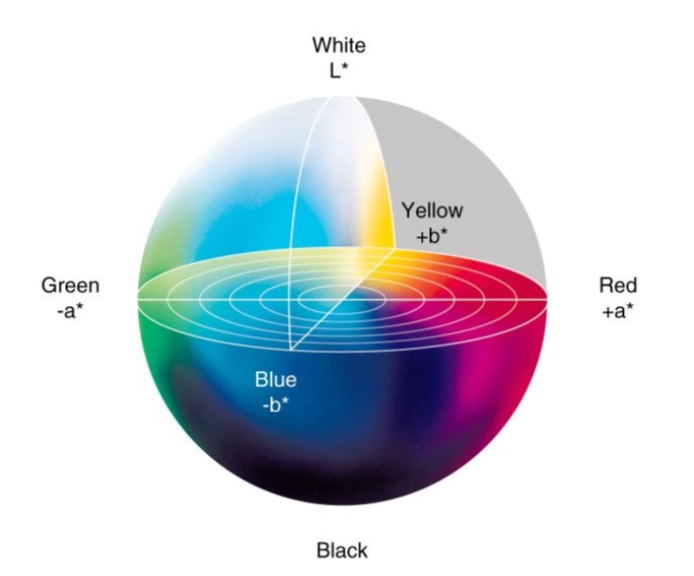
\includegraphics[width=170pt]{img/cielab.jpg}
  \caption{CIE Lab Color Space}
  \label{fig:cielab}
\end{figure}

\begin{equation}\label{DeltaE}
	\Delta E_{ab}= \sqrt{(L_{2}-L_{1})^2+(a_{2}-a_{1})^2+(b_{2}-b_{1})^2}
\end{equation}	
\\ In particular, from the result above it is possible to infer as follow:
\begin{itemize}
	\item when $0<\Delta E_{ab}<1$ an observer does not notice the difference;
	\item when $1\leq\Delta E_{ab}<2$ only experienced observers can notice the difference;
	\item when $2\leq\Delta E_{ab}<3.5$ unexperienced observers also notice the difference;
	\item when $3.5\leq\Delta E_{ab}<5$ clear difference in color is noticed;
	\item when $\Delta E_{ab}>5$ an observer notices two different colors.
\end{itemize}
\section{Resolution of Part 1}
The following section explains the choices you make in implementing the first part of the project.

\subsection{Dataset Reduction} 
The dataset is made up of 1269 samples of colors named "master" provided as a spectrum vector at a wavelength of 380nm to 800nm, the wavelenght of visible light. From these masters, distorted copies will need to be generated and then calculate the difference between the original colors and the copies as required by the project. It is possible to see (figure \ref{fig:dataset}), through a visual analysis of the dataset, that many master colors are "similar to each other" so the first operation was to skim the dataset by reducing the number of master colors. This helps reduce the computational cost of operations at first. In the next step, you will use the entire dataset. The solution used to reduce the dataset is to use the formula \ref{DeltaE} and eliminate the colors that have a difference between them, in terms of Lab coordinates, less than 3. After the reduction the number of samples in the dataset are 259 and the final dataset is shown in figure \ref{fig:reducteddataset}.
\begin{figure}
  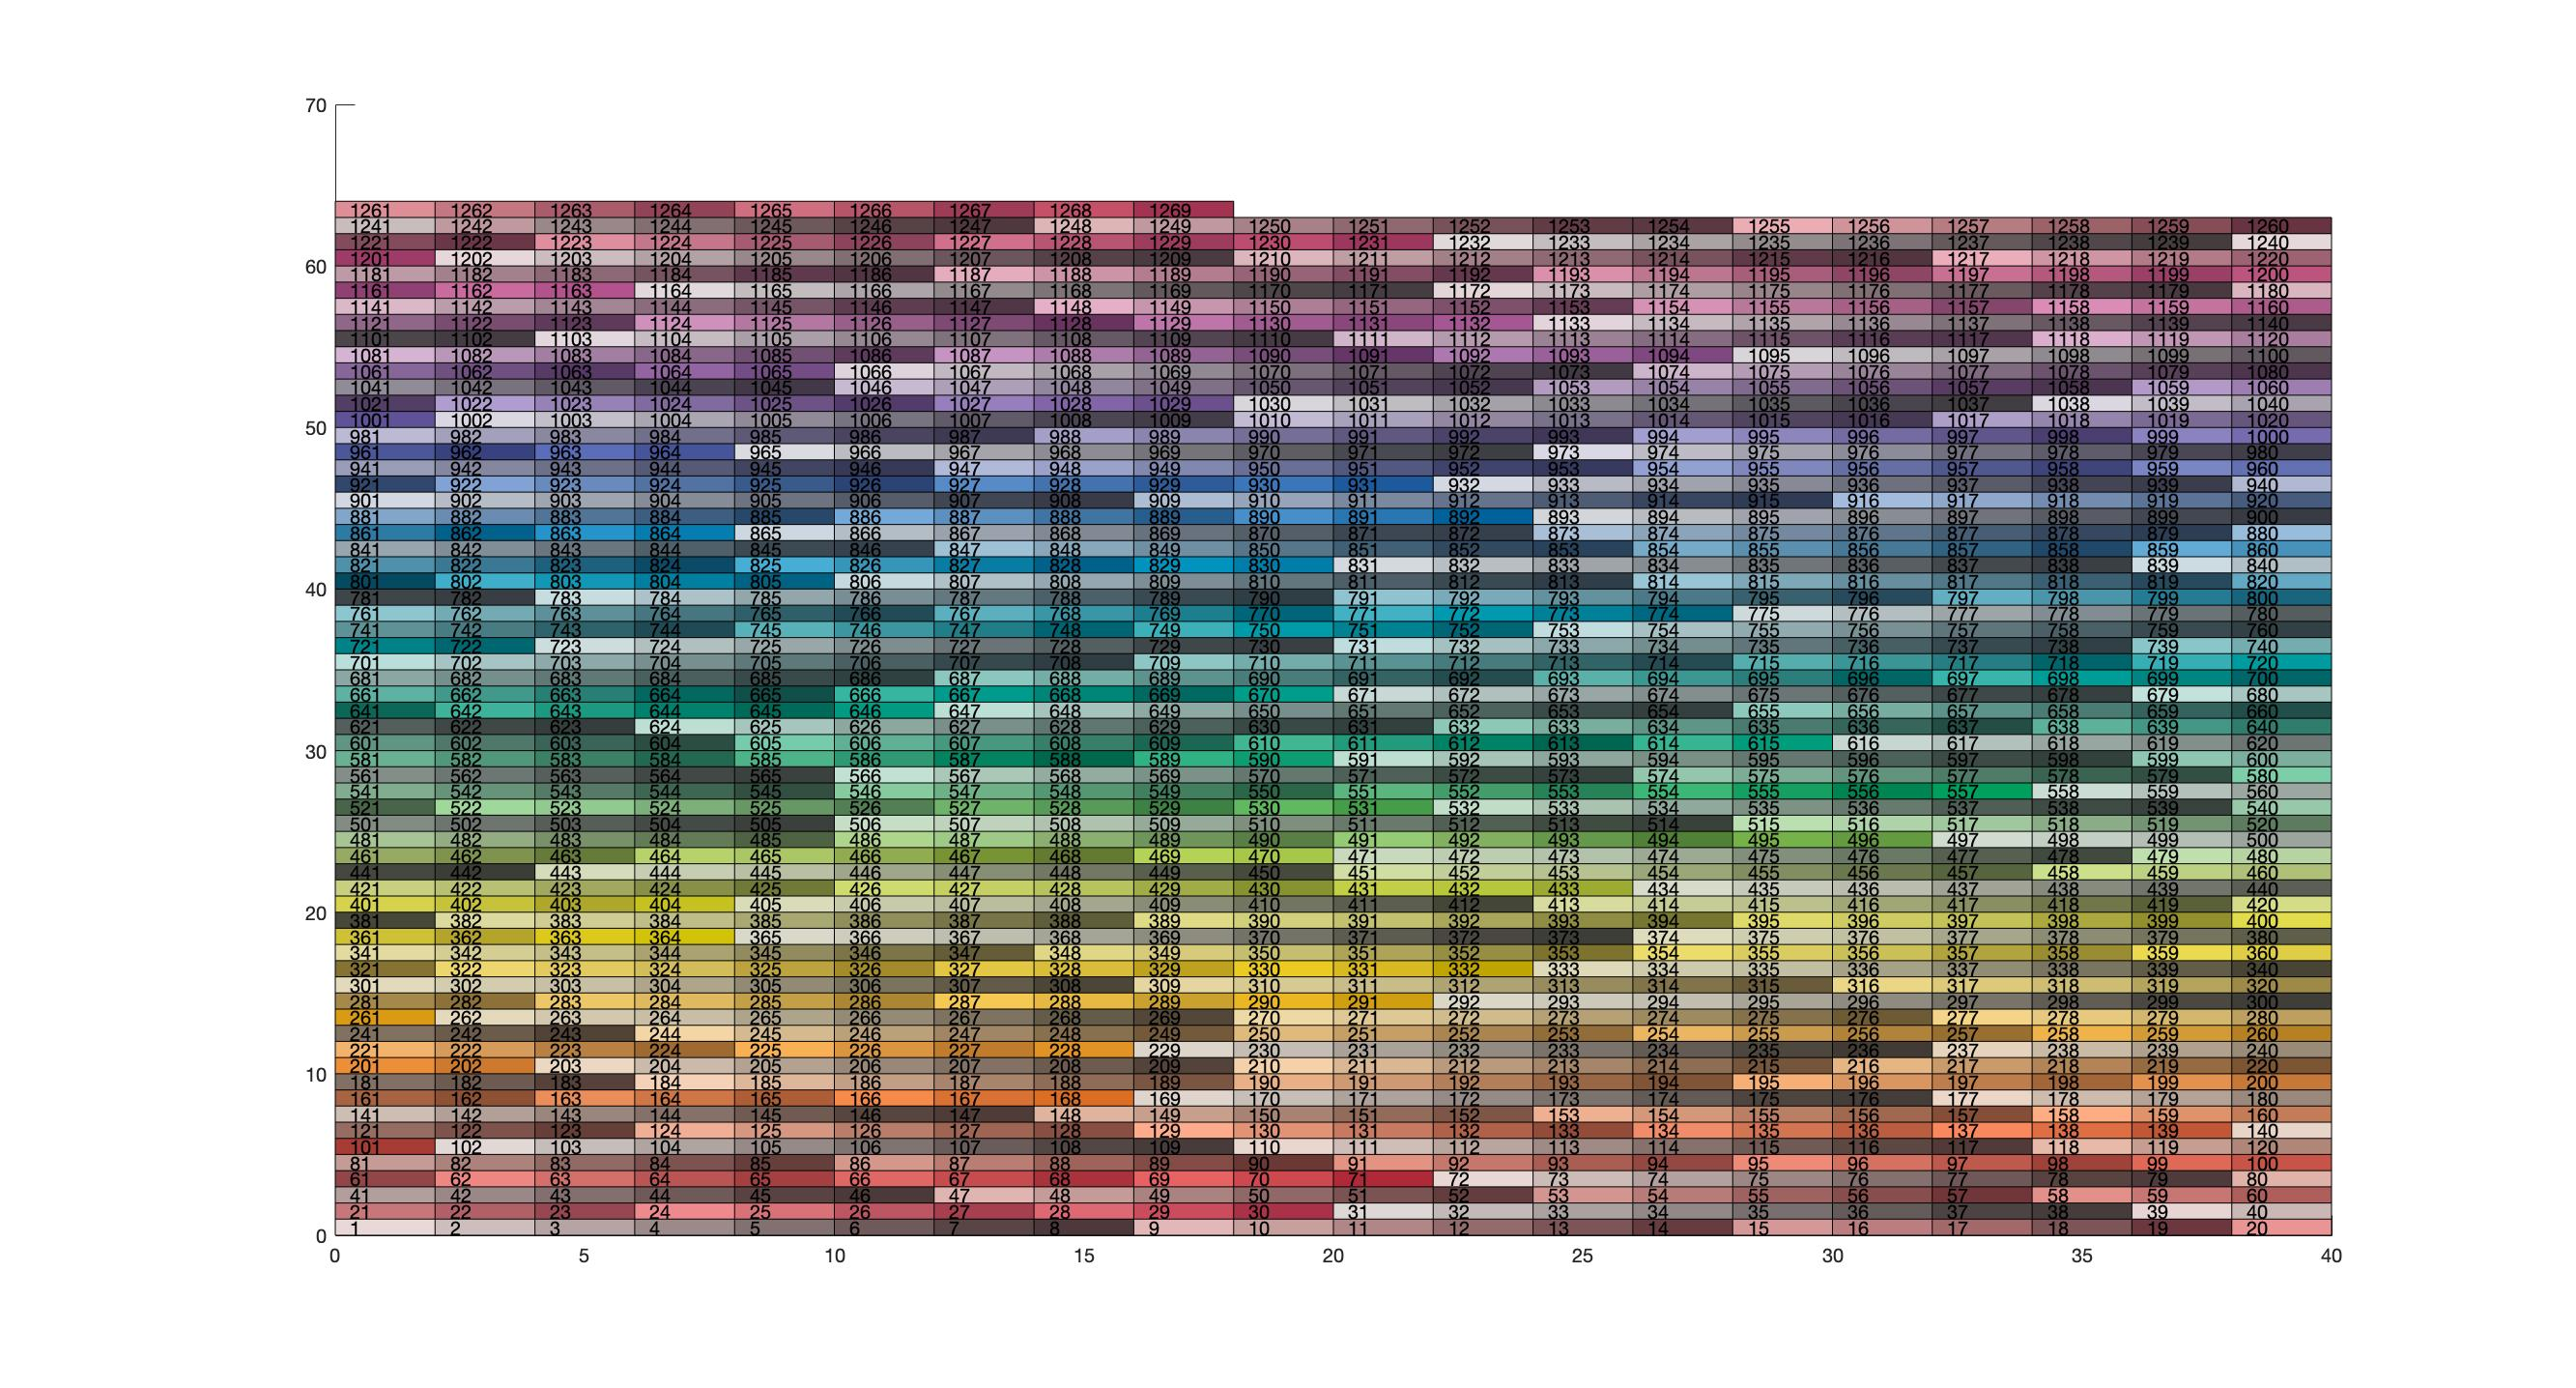
\includegraphics[width=\linewidth]{img/dataset.jpg}
  \caption{Original Dataset}
  \label{fig:dataset}
\end{figure}
\begin{figure}
  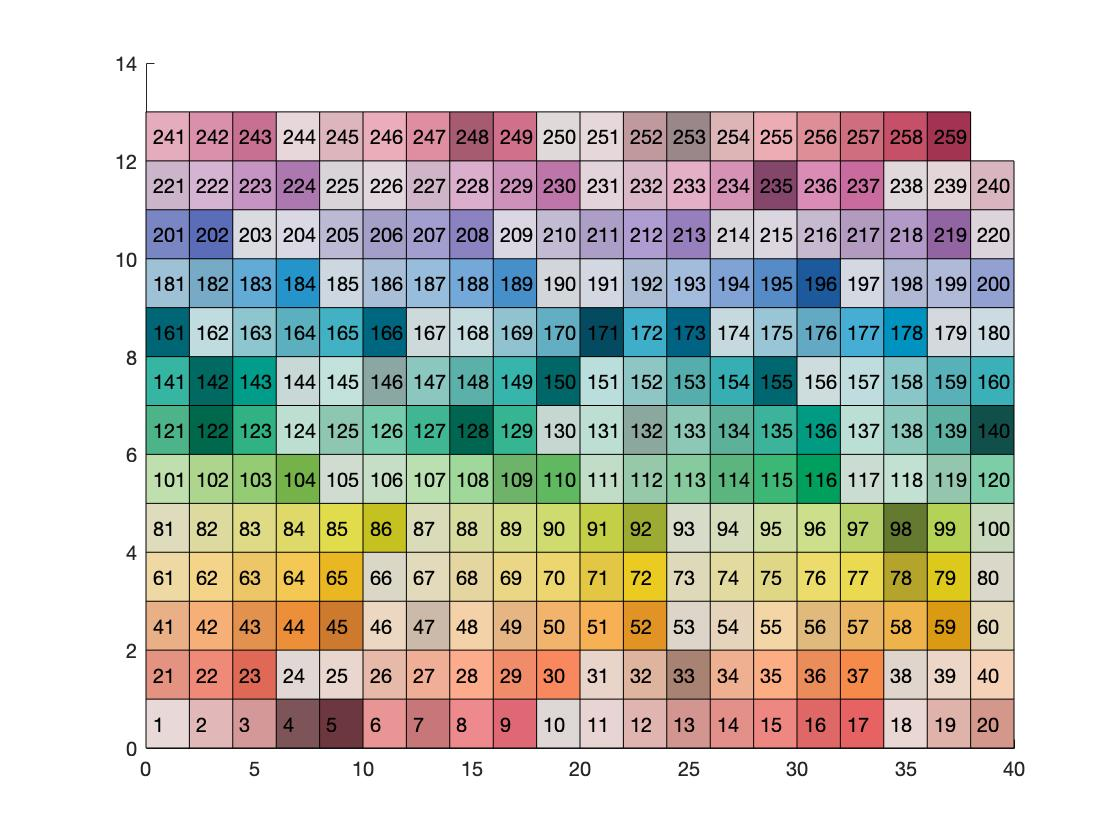
\includegraphics[width=\linewidth]{img/reducteddataset.jpg}
  \caption{Reduced Dataset}
  \label{fig:reducteddataset}
\end{figure}
\subsection{Copy Creation} 
For the aim to create an homogeneus dataset
The hypothesis used for the creation of the copies is the follow one: since the reference context is an industrial process, it is difficult to have a color difference greater than 5 i.e. a $\Delta E>5$. A script (noiseInterval.m) then evaluated the noise interval that could keep the low percentage of copies with $\Delta E>5$ but not negligible (for the purpose of the creation of an homogeneous dataset). Starting from an absent noise i.e. with a factor of 1, noise intervals were analyzed by increasing noise factor by 0.01. Table \ref{tab:tablepercentage} shows the results. The noise factor used is 1.18 and the range therefore varies randomly in [1,1.18]. To obtain a distortion of the spectrum, and then a copy, it is chosen to multiply the spectrum by a noise factor. An example can be shown in Figure \ref{fig:mastercopy} . The generation of copies was achieved by running the script \textbf{makeMasterCopyMatrix.m} that generated a number of 10 distorted copies for each master color in a noise range ranging from [1.00,1,18].
\begin{table}[h!]
  \begin{center}
    \label{tab:tablepercentage}
    \begin{tabular}{c|c|c|c|c|c} 
      \textbf{Interval} & \textbf{$0<\Delta E<1$} & \textbf{$1\leq\Delta E<2$}&\textbf{$2\leq\Delta E<3.5$}&\textbf{$3.5\leq\Delta E<5$}&\textbf{$\Delta E\geq5$}\\
       \hline
      $[1;1.12]$ & 0.25	 &0.29	&0.38	&0.07	& 0\\
      $[1;1.13]$ & 0.23 &	0.27 &	0.37 &	0.13 & 	0\\
      $[1;1.14]$ & 0.25 & 0.24 & 	0.33 &	0.18 &	0.001\\
      $[1;1.15]$ & 0.21 &	0.23 &	0.34 &	0.21 &	0.01\\
      $[1;1.16]$ & 0.21 &	0.21 &	0.31 &	0.24 &	0.03\\
      $[1;1.17]$ & 0.20 &	0.20 &	0.30 &	0.24 &	0.06\\
      $[1;1.18]$ & 0.19 &	0.18 &	0.28 &	0.25 &	0.10\\
      $[1;1.19]$ & 0.17 &	0.18 &	0.26 &	0.26 &	0.13\\
    \end{tabular}
    \caption{Percentage of Value in an interval of noise factors}
  \end{center}
\end{table}

\begin{figure}[h]
\center
  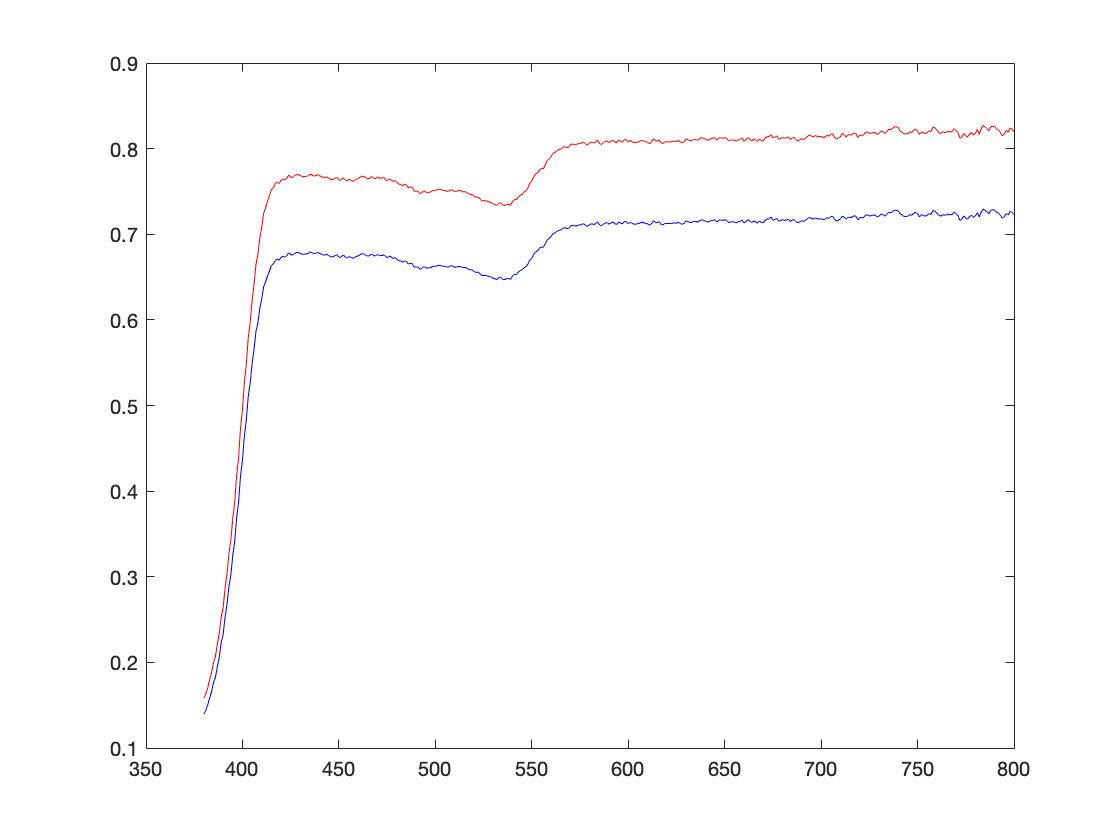
\includegraphics[width=300pt]{img/mastercopynoise.jpg}
  \caption{Master Color and Distorted Copy}
  \label{fig:mastercopy}
\end{figure}




\subsection{Feature Extraction} 
Since the inputs of the neural network are represented by the 421 components of the master spectrum and 421 of the copy spectrum, a reduction in the number of inputs is necessary since 842 inputs are too much. The basic idea adopted in this project is to divide the spectra into intervals and calculate for each range the features to be proposed as input to the network. The first features chosen for each range were the standard statistical indexes: \textbf{Mean, Median, Maximum, Minimum, Variance and Standard Deviation} as shown in Figure \ref{fig:features}.Since the mathematical \textbf{standard deviation} is the square root of the variance it was decided not to insert it in the characteristics since for the network it could be a redundant information (there is a very strong correlation about the two features). After many experiments with statistical indexes the number of inputs has been reduced considerably with good performance. For example with a number of 10 intervals the inputs go from 842 to 120 with an 86\% gain in terms of number of inputs. After this process, through the feature selection phase it is possible to optimize this gain even more. However, this approach has been discarded since it is possible to do even better with the following one.
If you take into consideration the only average of each interval, you can reconstruct the original spectrum and also remove the noise (as shown in Figure \ref{fig:interpolation}). \\
\textbf{In practice we tried to understand if the only averages are sufficient to characterize the entire original spectrum.}
The first question to answer is what is the number of intervals.
The choice of the number of intervals was made according to the following criterion: the spectrum is divided into intervals and the average is calculated for each interval. The new spectrum will have a number of values equal to the number of intervals. The new spectrum is interpolated (with a cubic interpolation) using the \textbf{interp1()} function of the Curve Fitting Toolbox and calculates how much interpolation differs from the original spectrum by the imse() function that calculates the mean squared error. If the value is very close to 0 then the interpolation represents a good approximation of the original function. In addition, the interval division also reduces the noise of the original spectra as shown in figure \ref{fig:interpolation} . After many experiments, the number of intervals chosen is 15 as the value of the average quadratic error settles into an order of magnitude ranging from 10\textsuperscript{-4} to 10\textsuperscript{-5} that is a very good result.

\begin{figure}[!h]
\center
  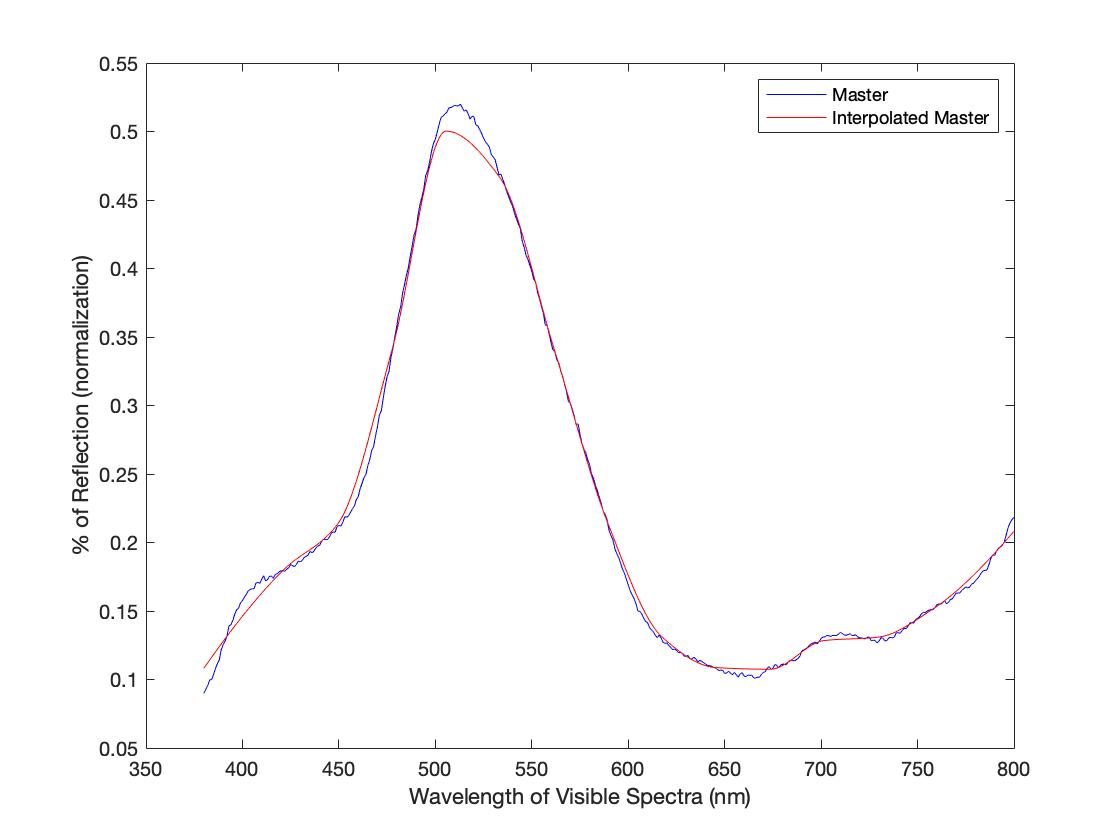
\includegraphics[width=300pt]{img/interpolation.jpg}
  \caption{Master Color and Interpolation}
  \label{fig:interpolation}
\end{figure}

\begin{figure}[!h]
\center
  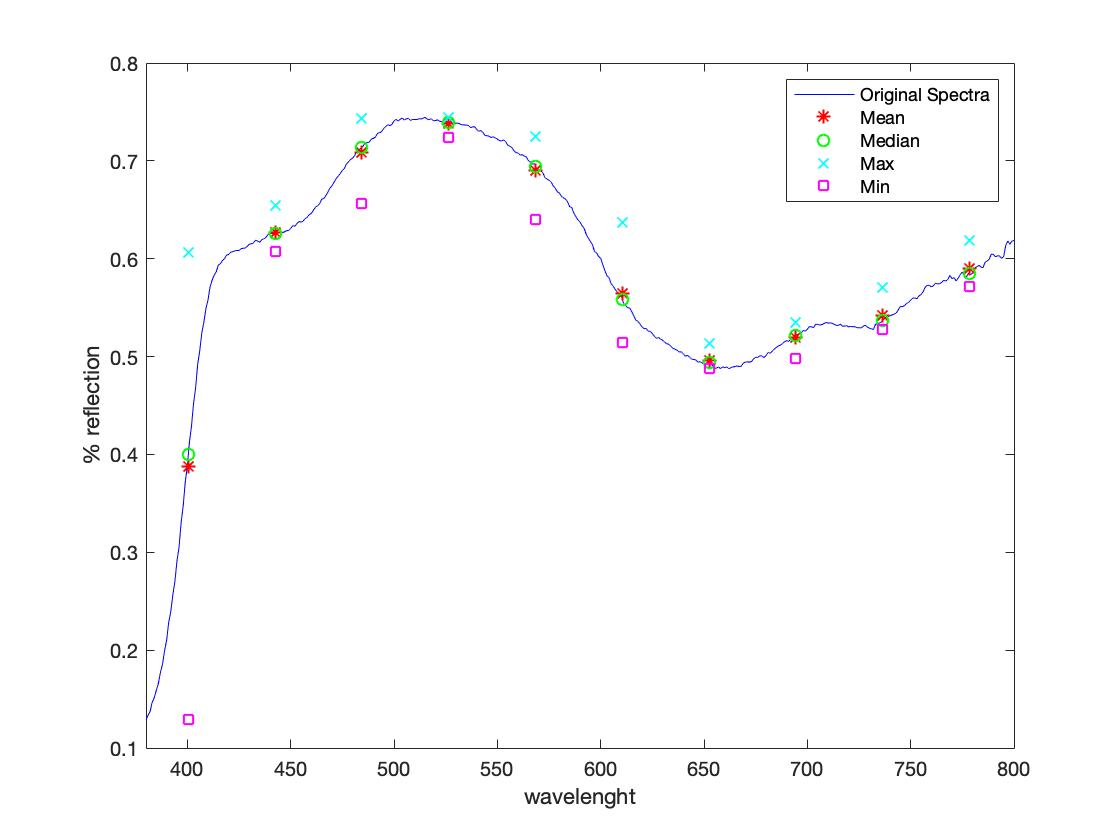
\includegraphics[width=300pt]{img/features.jpg}
  \caption{Features extracted from a spectra}
  \label{fig:features}
\end{figure}

\subsection{Feature Selection} 
After extracting the characteristics for each interval, it is possible to further decrease the number of inputs by selecting the characteristics. This selection was made through the selectionfs function. After numerous experiments, a correct tradeoff was chosen for the number of features extracted equal to 6. The stop criterion of the function was the performance of the neural network used for the selection of the characteristics and that is the mse. After many iterations and experiments the final columns included at the end are almost the same:  [ 1 7 16 22 ]. \textbf{In this way the number of inputs are reducted from 30 to 4}. 
 
\subsection{Setting the Neural Network} 
At this point in the project it is possible to use the inputs and targets as input of a shallow neural network for function fitting.
The choice of the implementation of the neural network is performed by creating a MATLAB network using the \textbf{fitnet()} function with a number of neurons equal to n and calculating the performance:
\begin{verbatim}
	hiddenLayerSize=n 
	net=fitnet(hiddenLayerSize);
	net.divideParam.trainRatio=70/100;
	net.divideParam.valRatio=15/100; 
	net.divideParam.testRatio=15/100; 
	net=train(net,inputs,targets);
\end{verbatim}
The performances are calculated starting from a number of hidden neurons equal to 1 and increasing it. This is done 10 times and network performance in terms of \textit{mean squared error} and \textit{training time} are calculated.The results of the experiment are shown in the following Table \ref{tab:tablefitnn}.From the results of the experiments it is possible to see that a good trade-off for the choice of the number of hidden neurons is represented by n = 4. 
\begin{table}[h!]
  \begin{center}
    \label{tab:tablefitnn}
    \begin{tabular}{c|c|c|c|c|c} 
      \textbf{No. Hidden Neurons} & \textbf{mse}&\textbf{Training Time}\\
       \hline
     1 	 &0.15	&0.30\\
     2	 &0.03&	0.98\\
     3	 &0.027	 &0.66\\
     4	 &0.010	 &0.72\\
     5	 &0.010& 1.3\\
    \end{tabular}
    \caption{Performances evaluated in Neural Network's Training}
  \end{center}
\end{table}
The randomness of the experiment repetitions is introduced by the 'dividerand' option of the MATLAB neural network toolbox. In this way the training, testing and validation sets are represented by different elements for each iteration. In general the choice of a greater number of hidden neurons involves more time for the traning and more samples are required. Having a greater number of neurons also results in a better fit and a better regression coefficient.
Adopting the results of the experiments and the choices made above the final network has a \textbf{regression coefficient equal to 0.9982 and an mse equal to 0.0103}. The value of the regression coefficient very close to 1 confirms that the fitting of the function is very good as show in figure \ref{fig:regression}.

\begin{figure}[!h]
\center
  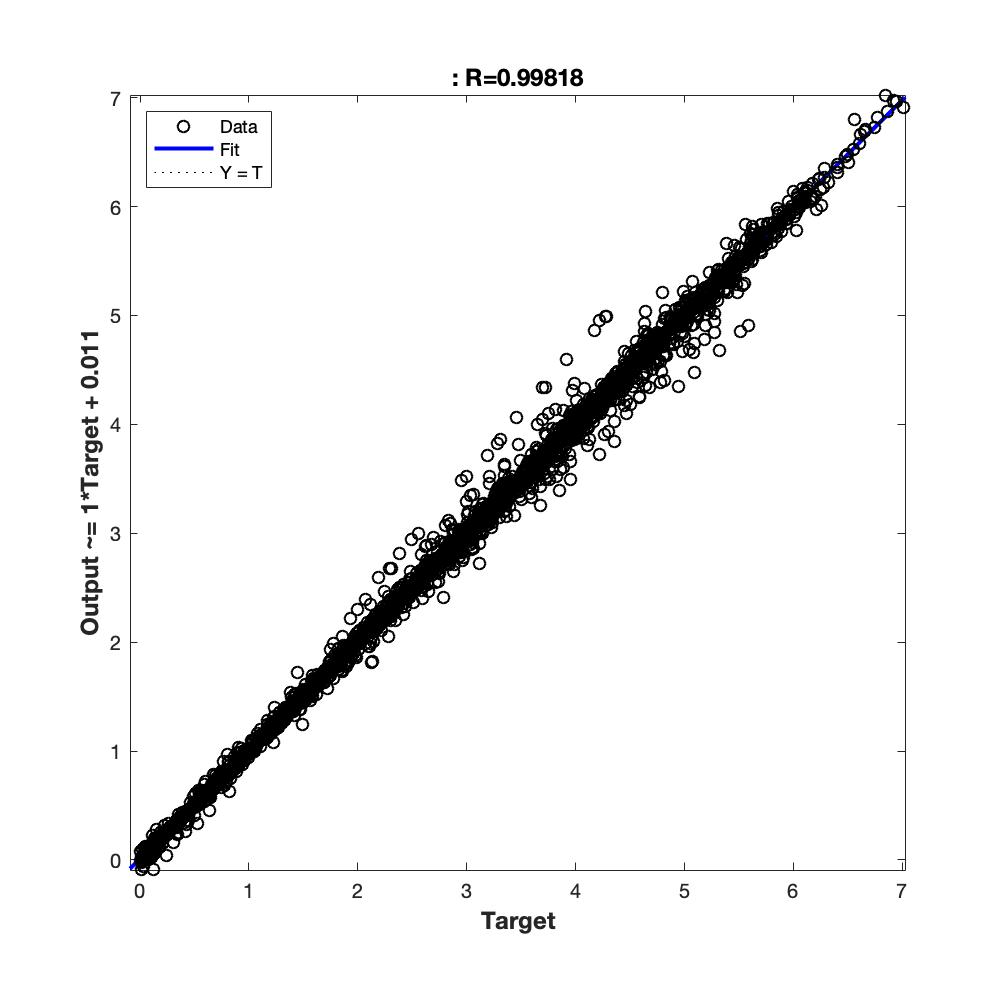
\includegraphics[width=300pt]{img/regression.jpg}
  \caption{Regression Plot of the Final Neural Network}
  \label{fig:regression}
\end{figure}

\newpage


\section{Project Description (Part 2) }
The purpose of the second part of the project is to produce a fuzzy system in order to correct any inaccuracies present using the formula to calculate the $\Delta E$ (formula \ref{DeltaE}). For this purpose, instead of the coordinates L*a*b*, the color space L*c*h* will be used use. The L*C*h colorspace (figure \ref{fig:clhcolorspace}), similar to CIELAB, is preferred by some industry professionals because its system correlates well with how the human eye perceives color. It has the same diagram as the L*a*b* color space but uses cylindrical coordinates instead of rectangular coordinates.
In this color space, L* indicates lightness, C* represents chroma, and h is the hue angle. The value of chroma C* is the distance from the lightness axis (L*) and starts at 0 in the center. Hue angle starts at the +a* axis and is expressed in degrees (e.g., 0° is +a*, or red, and 90° is +b, or yellow).\footnote{From: https://sensing.konicaminolta.us/blog/understanding-the-cie-lch-color-space/}. \\\\\\\\In particular this phase of the project is composed for three phases: 
\begin{itemize}
	\item\textbf{Detection of the imprecision areas:} We have to find the areas in che CIE L*a*b* affected by imprecisions in terms of mismatching between the analytical formula for compute $\Delta E$ and the observer's experience.
	\item\textbf{Setting a fuzzy system}: Build a fuzzy set for fix these imprecisions expressed in terms of fuzzy rules.
	\item\textbf{Correct the Output of the Original Expression}: Correct the output of the formula using the result of the fuzzy system that we created.
	\item\textbf{Train the neural network with the new adjusted data}: Train again the neural network built before with the adjusted data obtained from the fuzzy system as targets. 
\end{itemize}
	
	
\begin{figure}[!h]
	\center
 	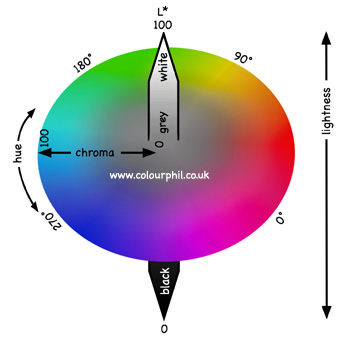
\includegraphics[width=200pt]{./img/lchcolor.jpg}
  	\caption{Simple schema for the L*C*h* Colorspace}\label{fig:clhcolorspace}
\end{figure}

\begin{figure}[!h]
	\center
 	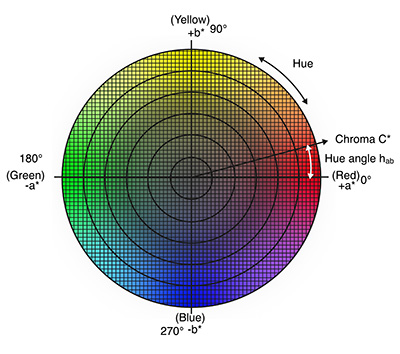
\includegraphics[width=200pt]{./img/ciecolordspace}
  	\caption{A slice of the L*a*b* color space at L*=50}\label{fig:ciecolordspace}
\end{figure}

\subsection{Detection of Imprecision Areas} 
The imprecision areas of the CIE L*a*b* color space are such as to provide a $\Delta E$ difference between two colors that does not reflect, in numerical terms, the real experience of an external observer. The inaccuracy areas and their corrections to be made are described below.
\subsubsection{Dark Colors}
When two colors are dark (see figure \ref{fig:dark}, also if they belong to different hues, an external observer doesn't notice a clear difference. An example is shown on the figure X. Two colors having a $\Delta E$=8 are different colors as we said in the first part of the project. An observer instead perceive a very smaller difference than $\Delta E$ of the formula \ref{DeltaE} . The value of $\Delta E$ has to be very small.
\subsubsection{Yellow Area}
When two colors belongs to the Yellow Area a similar behaviour occurs. The value of the $\Delta E$ obtained from the analytical formula is higher than it should be how it's possible to see in the figure X. The value of $\Delta E$ has to be smaller.
\subsubsection{Blue/Violet Area}
When two colors belongs to the Blue/Violet Area instead an external observer notices an higher difference of the colors than the one expressed from the formula $\Delta E$ (see figure X). In this case the $\Delta E$ has to be higher.
\subsubsection{Unsaturated Colors}
When two colors belongs to the area of the unsaturated colors they could belongs to really different hue so they could be really differents. The anylitical formula suggests to have a small $\Delta E$ but the real experience suggests that the $\Delta E$ has to be higher because an external observer notices an higher difference also if the colors are unsatured as shown in the figure X.
\subsection{Setting a fuzzy system} 
From the project specifications the fuzzy network where to receive the L*c*h* coordinates of the master color as input, to understand in which Lab area it belongs, and the original $\Delta E$ generated by the formula \ref{DeltaE}. As output, instead, you will have the correct $\Delta E_{corr}$.
The purpose of this phase of the project is to create fuzzy sets with membership function for the 4 inputs and for the output. Next we define the rules that link the inputs to the output to get the correct $\Delta E_{corr}$ that will become a new input for the neural netwrok we built in the first part of the project.
\subsubsection{Luminosity}
From the CIE definition (figure \ref{fig:ciecolordspace}) the Luminosity $L\in[0:100]$ and the relative fuzzy set is shown in the figure \ref{fig:luminosity} .

\begin{figure}[!h]
	\center
 	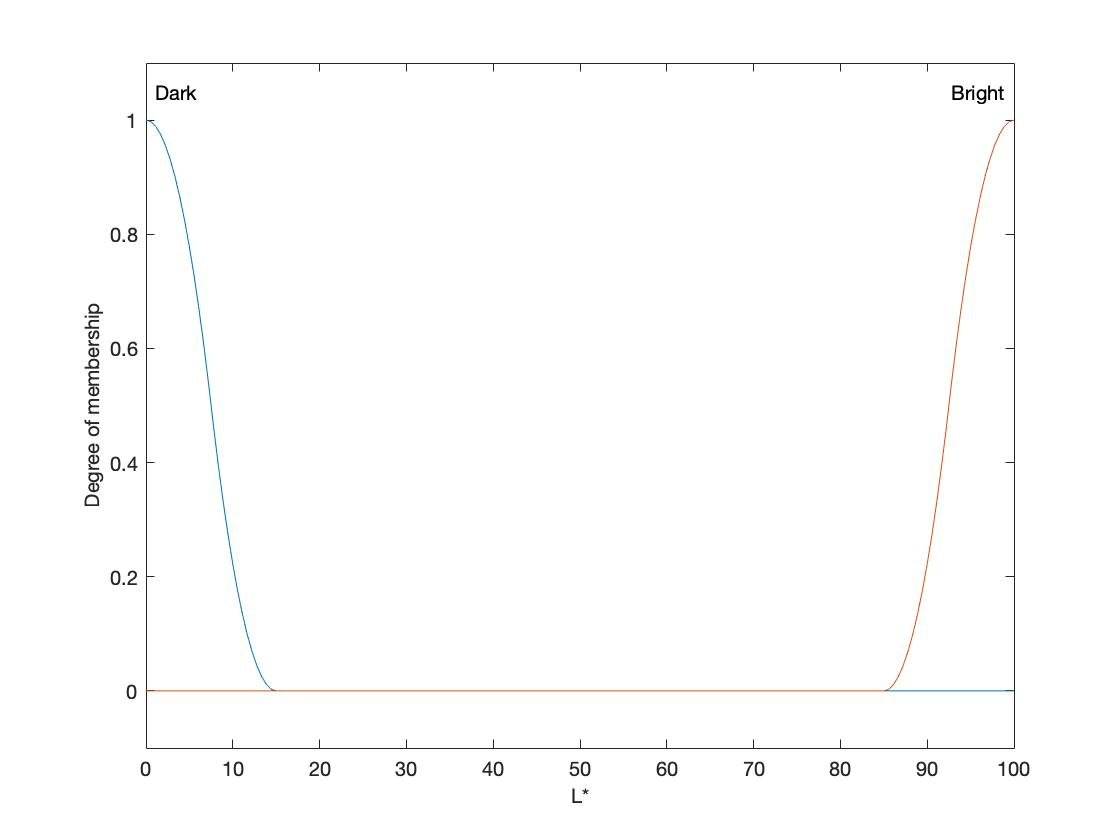
\includegraphics[width=300pt]{./img/inputFuzzyL}
  	\caption{Luminosity Membership Function}\label{fig:luminosity}
\end{figure}

\subsubsection{Hue}
From the CIE definition the Hue $H\in[0:360]$ in terms of degrees as shown in the figure \ref{fig:ciecolordspace} and the relative fuzzy set is shown in the figure \ref{fig:hue} .

\begin{figure}[!h]
	\center
 	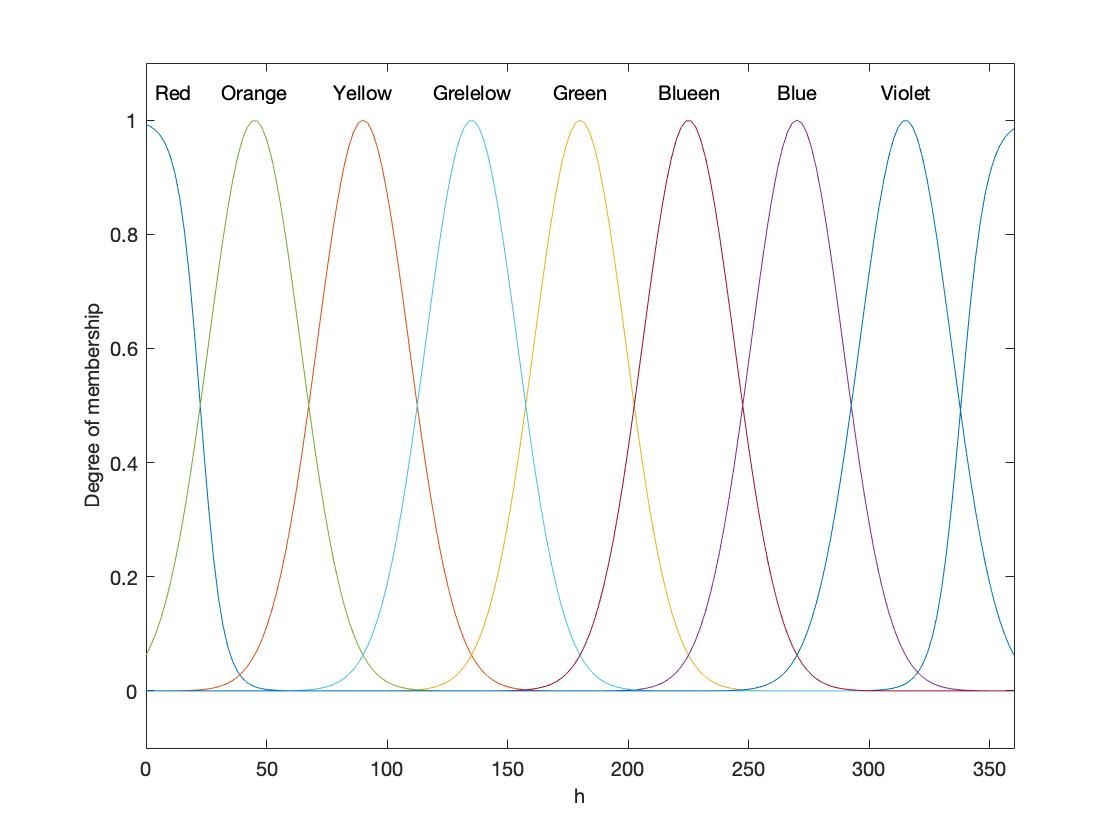
\includegraphics[width=300pt]{./img/inputFuzzyH}
  	\caption{Hue Membership Function}\label{fig:hue}
\end{figure}

\subsubsection{Chroma}
From the CIE definitions it's possible to notice that the parameter C belongs to the range [0 : $C_{max}$]. Where $C_{max}\approx{127}$ at L=50 as shown in the figure \ref{fig:ciecolordspace}.
The main problem is that the above value $C_{max}$ is relative to the value of L* so we will call it $C_{1max}$. If we manage the color space as an ellipse (equation \ref{fig:ellipse}) is it possible to obtain the value of $C_{1max}$ (equation \ref{fig:cmax}) and the final value $c_{perc}$ that express the c* as a percentage. In this way we can have an input value for the fuzzy system belonging as $c_{perc}\in[0:100]$. The relative fuzzy set is shown in figure \ref{fig:Chroma}.


\begin{equation}\label{fig:ellipse}
	x^2/C_{max}^2 + y^2/C_{max}^2 + (l-50)^2/50^2=1
\end{equation}	

\begin{equation}\label{fig:cmax}
	C_{1max}^2= x^2 + y^2 =C_{max}^2 * (1- (l-50)^2/50^2)
\end{equation}	

\begin{equation}\label{fig:cperc}
	c_{perc}=100*c/C_{1max}
\end{equation}

\begin{figure}[!h]
	\center
 	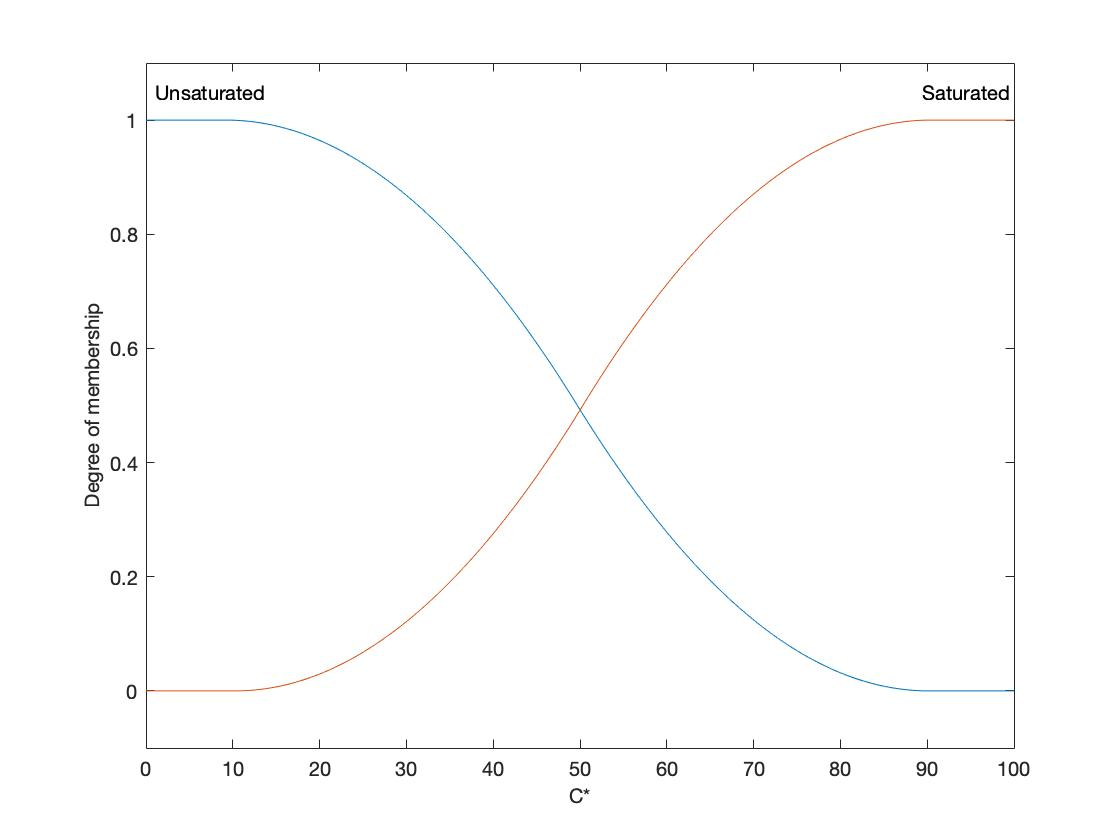
\includegraphics[width=300pt]{./img/inputFuzzyCperc.jpg}
  	\caption{Chroma Membership Function}\label{fig:Chroma}
\end{figure}

\subsubsection{The input $\Delta E$ and the output $\Delta E_{corr}$} 

For what concern the input $\Delta E$ (obtained from the formula \ref{DeltaE}) and the output $\Delta E_{corr}$ of the Fuzzy System, the relative fuzzy set is the same and is the one in figure \ref{fig:deltaemf}.

\begin{figure}[!h]
	\center
 	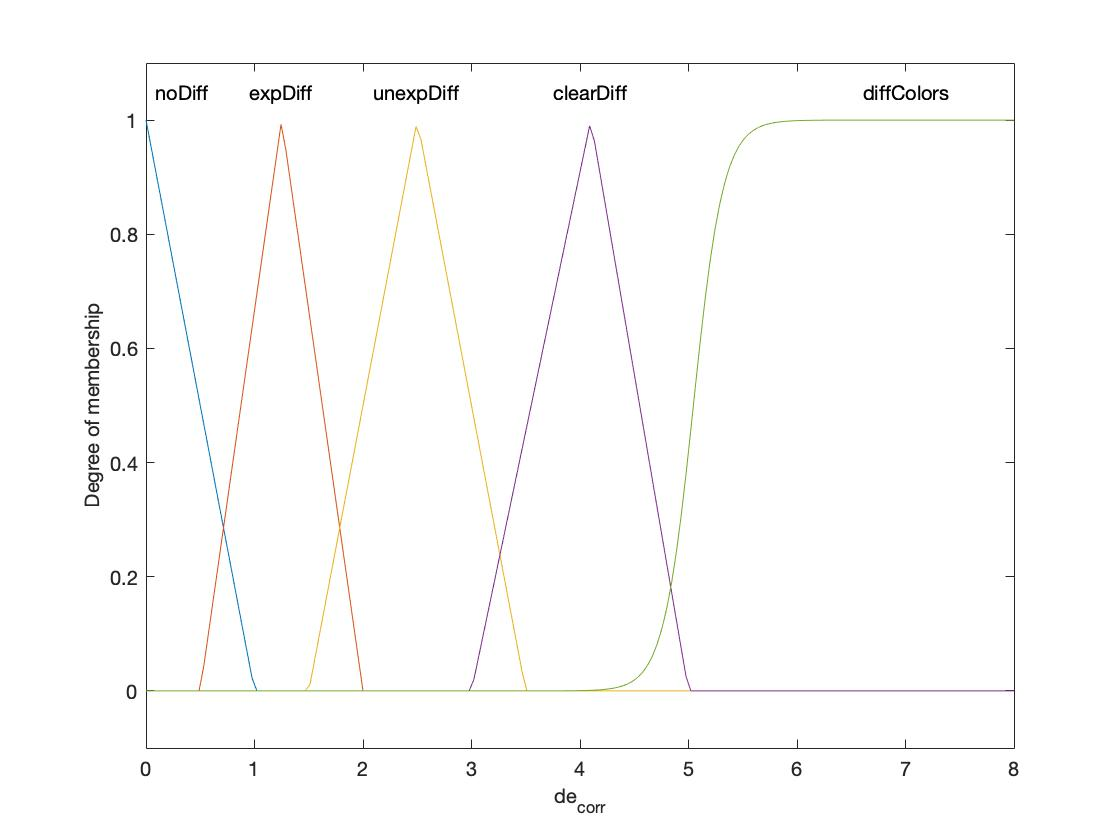
\includegraphics[width=300pt]{./img/outputFuzzyDelta}
  	\caption{$\Delta E$ Membership Function}\label{fig:deltaemf}
\end{figure}

\subsection{Correct the Output of the Original Expression} 

At this point of the project, for fix the inaccuracies of the original formula for compute the $\Delta E$ (formula \ref{DeltaE}) a set of fuzzy rules is elaborated as shown in the figure \ref{tab:fuzzyrules}.
With this set of rules we can compute a $\Delta E_{corr}$ that will represent a new target vector for the neural network built above.
Furthermore we decide to create a function that check which input don't match with the fuzzy rules. In this way the fuzzy system will not affect, for example setting a default value, the input that don't need to be fix.

\begin{table}[h!]
  \begin{center}
    \label{tab:fuzzyrules}
    \begin{tabular}{c|c|c|c|c|c} 
      $L*$&$c_{perc}$*&$h*$&$\Delta E$&$\Delta E_{corr}$\\
       \hline
     Dark &-&-&-&noDiff\\
     not Dark &unsatured&-&expDiff&unexDiff\\    
     not Dark &unsatured&-&unexpDiff&clearDiff\\   
     not Dark &satured&yellow&unexpDiff&expDiff\\   
     not Dark &satured&yellow&clearDiff&unexpDiff\\   
     not Dark &satured&yellow&diffColors&clearDiff\\   
     not Dark &satured&blue&expDiff&unexpDiff\\   
     not Dark &satured&blue&unexpDiff&clearDiff\\   
     not Dark &satured&violet&expDiff&unexpDiff\\   
     not Dark &satured&violet&unexpDiff&clearDiff\\   

     \end{tabular}
    \caption{Fuzzy Rules for the Fuzzy System}
  \end{center}
\end{table}


\subsection{Train the neural network with the new adjusted data} 

In this last part the neural network built in the first part of the project is trained again with the $\Delta E_{corr}$ as a new target. The average performance in 10 repetition of training are represented from a \textbf{regression coefficient equal to 0.9739 and an mse equal to 0.0542}. Better performance (comparable with the neural network trained in the first part of the project) can be achieve increasing significatively the number of the hidden neurons $\approx{30}$ but with also a significatively increasing in the training process not reasonable since the regression coefficient is still excellent.

\subsection{Conclusions} 
How it's possible to see from the latest figures the new output of the neural network fix the inaccuracies we discussed about the formula \ref{DeltaE}. In particular from the figures \ref{fig:dark} and \ref{fig:yellow} is possible to check that the $\Delta E_{corr}$ is smaller than the previous $\Delta E$ in the dark and yellow areas. In the opposite side is possible to check that the $\Delta E_{corr}$ is higher than the previous $\Delta E$ in the blue and unsaturated areas (figures \ref{fig:unsaturated} and \ref{fig:violet}).
\begin{figure}[!h]
	\center
 	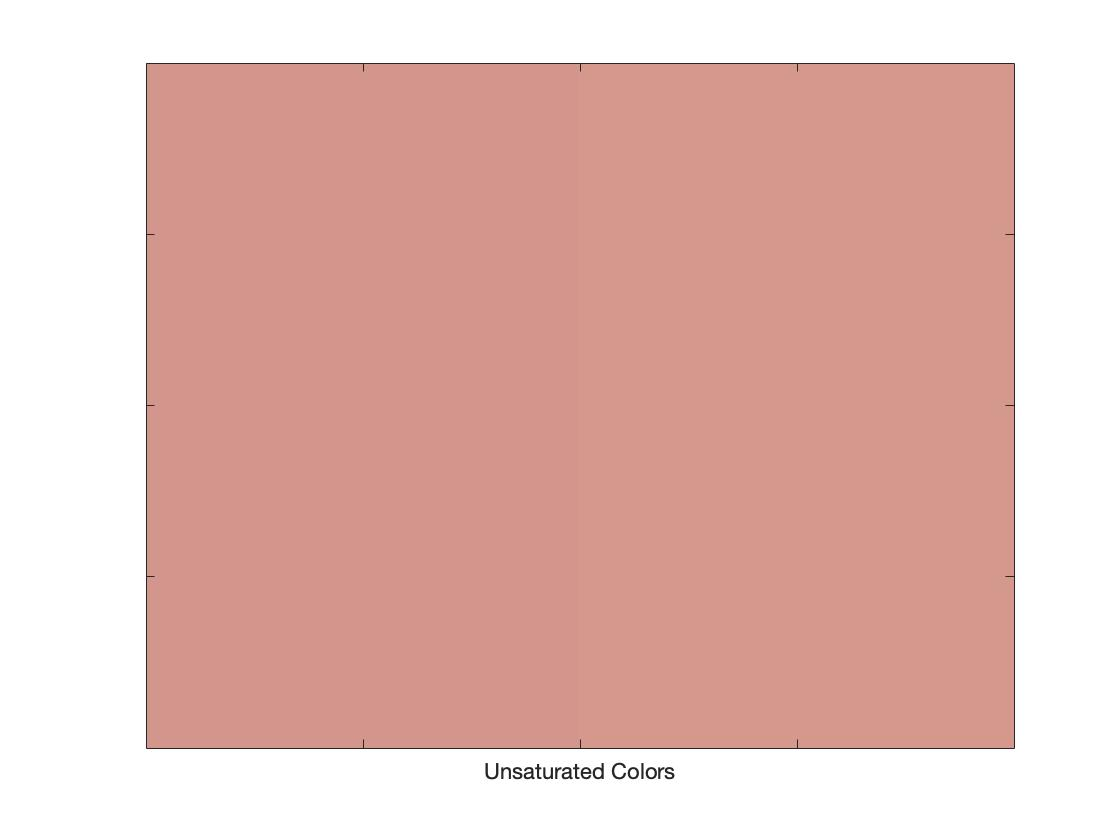
\includegraphics[width=300pt]{./img/unsaturated.jpg}
  	\caption{$\Delta E$=0.50  $\Delta E_{corr}$=1.40 }\label{fig:unsaturated}
\end{figure}
\begin{figure}[!h]
	\center
 	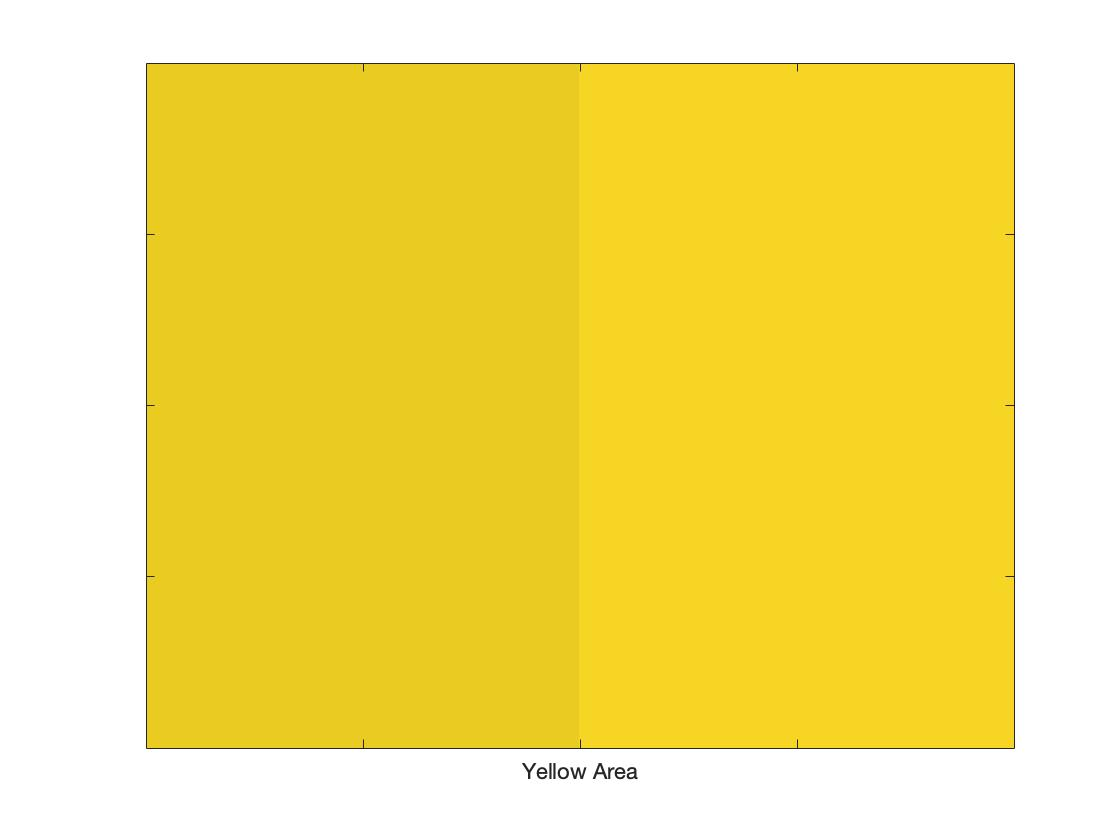
\includegraphics[width=300pt]{./img/yellow.jpg}
  	\caption{$\Delta E$=3.43  $\Delta E_{corr}$=2.57 }\label{fig:yellow}
\end{figure}
\begin{figure}[!h]
	\center
 	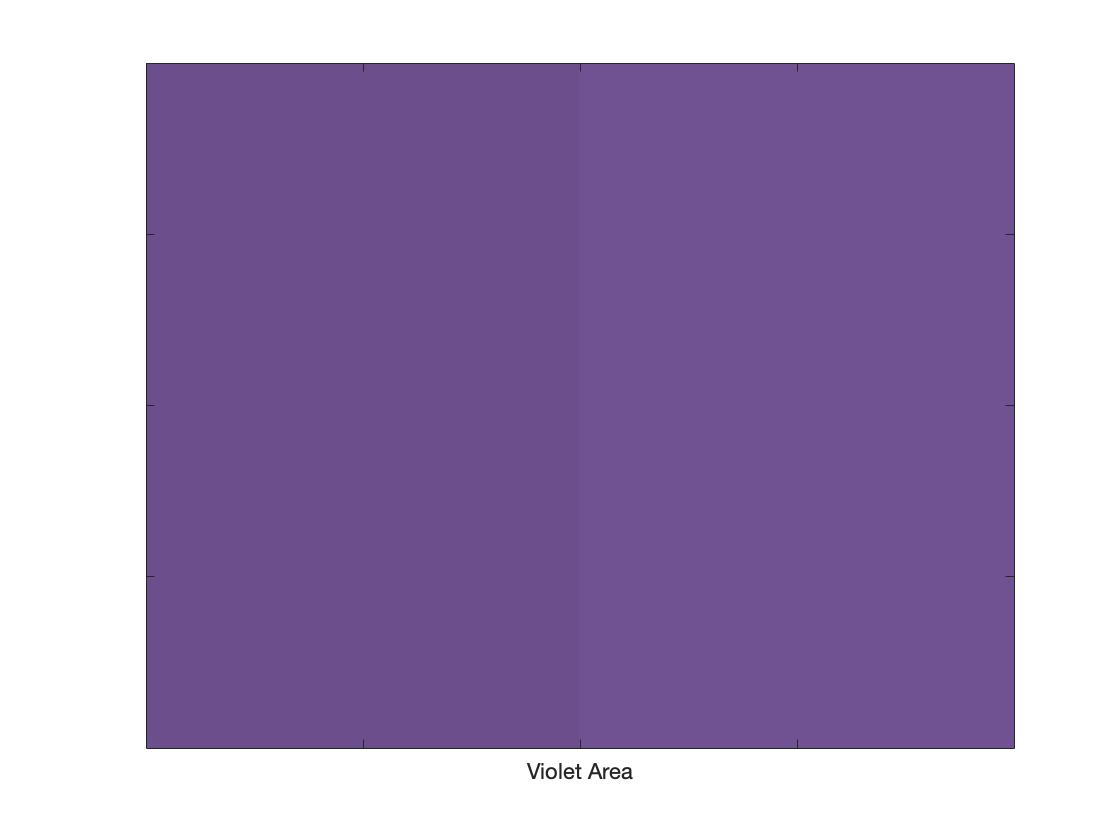
\includegraphics[width=300pt]{./img/violet.jpg}
  	\caption{$\Delta E$=1.73  $\Delta E_{corr}$=2.77 }\label{fig:violet}
\end{figure}

\begin{figure}[!h]
	\center
 	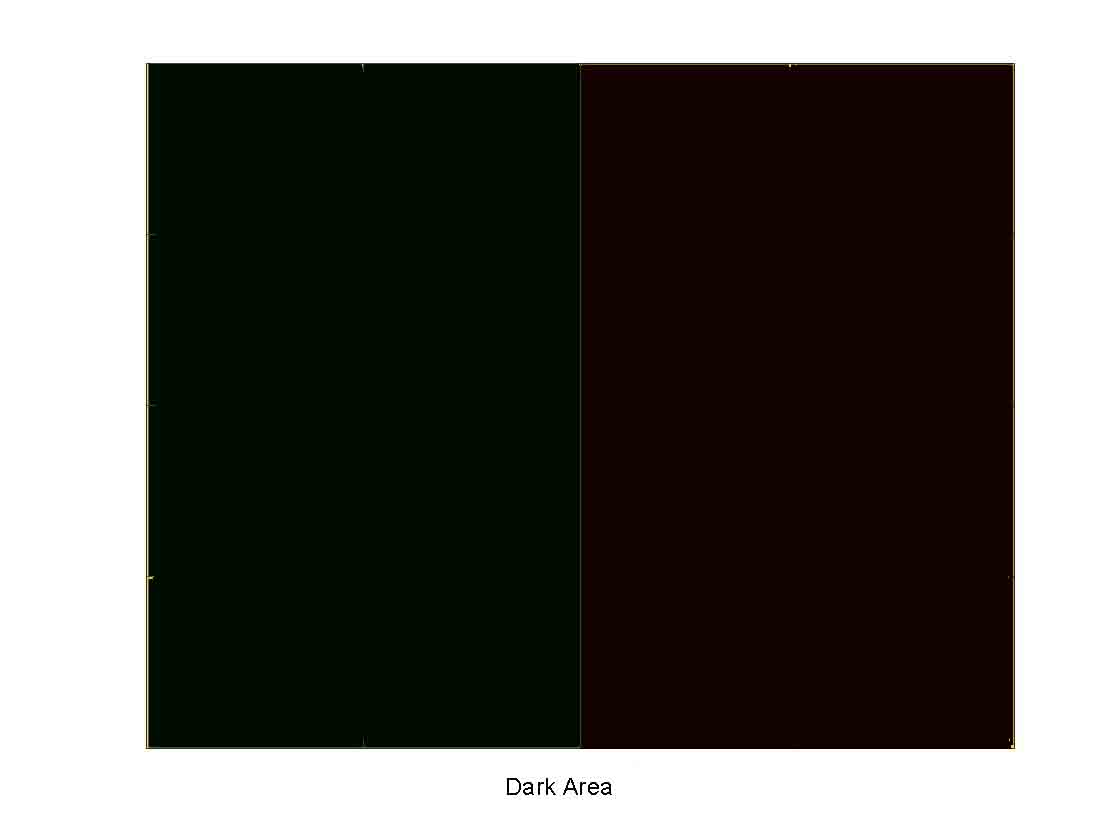
\includegraphics[width=300pt]{./img/dark.jpg}
  	\caption{$\Delta E$=4.30  $\Delta E_{corr}$=1.8 }\label{fig:dark}
\end{figure}






\end{document}



